\chapter{Binary Decision Diagrams}
\label{chap:bdd}

A Binary Decision Diagram (BDD) is an abstract data type representing a Boolean function, offering convenient
creation, manipulation, and analysis of Boolean functions in symbolic form \cite{bdds}. A BDD is a directed acyclic
graph structure widely used in formal design verification, test generation, and logic synthesis that provides an
algorithmic basis for symbolic model checkers \cite{bfs-bdd, bdds}.

A BDD is a collection of nodes (or vertices) interconnected with each other by links (or edges). In a BDD, leaf nodes
are called terminal nodes and are labeled with the Boolean values 0 and 1. The non-terminal nodes are referred to as
inner nodes. Each inner node is labeled with a Boolean variable $x_i$. An inner node has exactly two outgoing links:
a low link and a high link. When traversing the BDD, the chosen link depends on the valuation of $x_i$, $v(x_i)$. A
low link corresponds to $v(x_i)=0$ while high link to $v(x_i)=1$.

A simple BDD representing a single variable $x$ is depicted in Figure \ref{fig:simple-bdd}. The BDD contains two
terminal nodes, $0$ and $1$, which are depicted as squares. As a convention, all inner nodes use circles. In this
case, there is a single inner node with variable $x$. The high links are marked with a solid line and low links with
a dashed line. For $v(x) = 0$, the low link is followed to the corresponding terminal node $0$.

\begin{figure}
    \centering
    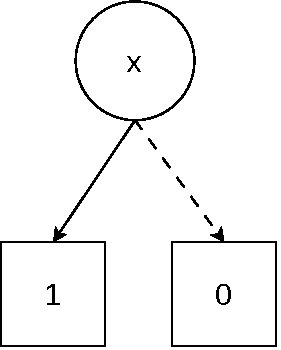
\includegraphics[width=0.2\linewidth]{figures/simple-bdd.pdf}
    \caption{The simplest BDD of a function $f(x)=x$}
    \label{fig:simple-bdd}
\end{figure}

Consider the following Boolean function:
\begin{equation}
    \label{eq:example}
    f(x_1, x_2, x_3) = (x_1 \land x_2) \lor x_3
\end{equation}

Function $f$ performs AND and OR on a vector of variables $X=(x_1, x_2, x_3)$. An example of a BDD representing this
function is portrayed in Figure \ref{fig:bdd}. In this case, the root node contains $x_2$. This particular BDD has
three interesting properties:

\begin{figure}
    \centering
    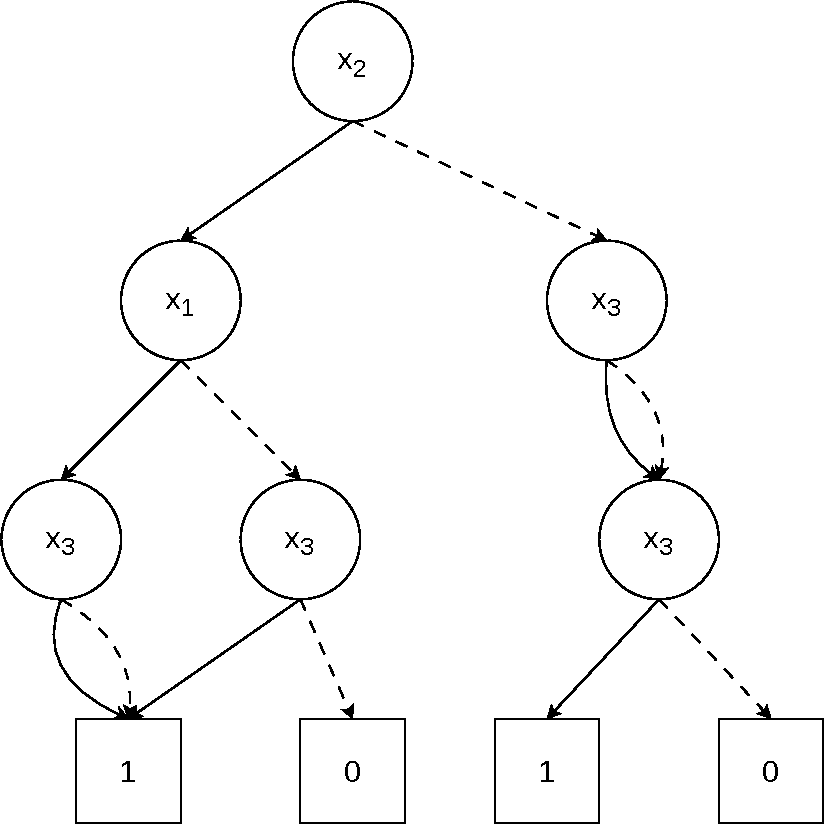
\includegraphics[width=0.6\linewidth]{figures/example-bdd.pdf}
    \caption{Binary Decision Diagram representing Boolean function $(x_1 \land x_2) \lor x_3$.}
    \label{fig:bdd}
\end{figure}

\begin{enumerate}
    \item Following only the high links from the root node, we will encounter an $x_3$ node with both of its links
        directed to the terminal node $1$. Similarly, the low link of $x_2$ also has both links directed to the same
        node. These are called \textit{redundant nodes}. \label{item:redundancy}
    \item There are two $x_3$ nodes with links to the terminal node $0$ and $1$. These are identical. Just like the
        two pairs of terminal nodes. \label{item:duplicate}
    \item The root node's high and low successors are $x_1$ and $x_3$ respectively. Following the low link leads to
        the aforementioned node $x_3$, which is again followed by node $x_3$. \label{item:ordering}
\end{enumerate}

While the BDD is correct, the graph is hard to read. Furthermore, these properties pose implementation challenges and
increase both time and space complexity of operations on this data structure. To address these three issues, let's
introduce some restrictions to a BDD.


\section{Types of BDDs}
\label{chap:bdd:types}

The points mentioned above lay the foundation for this section. An \textit{Ordered BDD} in subsection
\ref{chap:bdd:types:obdd} is a solution to point \ref{item:ordering}. Points \ref{item:redundancy} and
\ref{item:duplicate} are addressed by a \textit{Reduced Ordered BDD} described in subsection
\ref{chap:bdd:types:robdd}.


\subsection{Ordered BDD}
\label{chap:bdd:types:obdd}

The point \ref{item:ordering} outlines variables scattered in a seemingly random order. This makes the layer-by-layer
Breadth-first processing more challenging. An OBDD enforces a fixed variable ordering restriction. Let's assume a
total ordering of variables $x_n < x_n+1 < \ldots < x_{n+k}$ where the variable of terminal nodes in this ordering is
assumed to be $\infty$, so that $\infty > x_{n+k}$ \cite{ruddy}. A fixed variable ordering guarantees that traversing
the BDD encounters the variables in a certain order. This new property allows the graph to be structured
level-by-level, with one level per variable. This enables level-wise memory management and breadth-first manipulation
algorithms \cite{bfs-bdd, oxidd}.

Figure \ref{fig:obdd} displays the function $f$ of (\ref{eq:example}) as an OBDD with the previously stated variable
ordering. It is evident that nodes with variables $x_1$ and $x_2$ have swapped places, and that the redundant node
with $x_3$ was eliminated because the ordering $x_3 \nless x_3$ was violated.


\begin{figure}
    \centering
    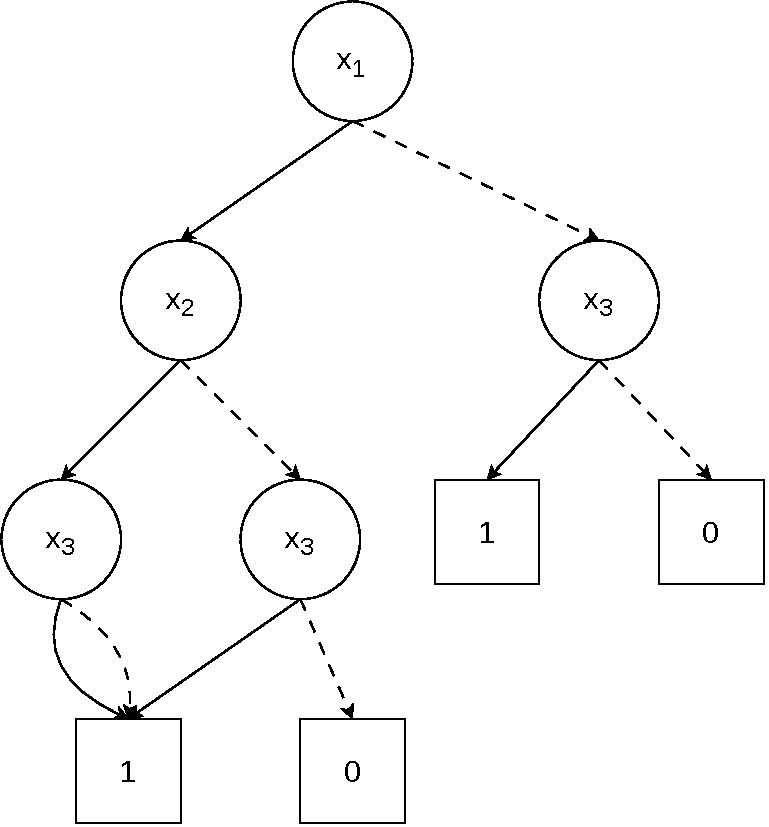
\includegraphics[width=0.6\linewidth]{figures/example-obdd.pdf}
    \caption{Ordered Binary Decision Diagram representing Boolean function $(x_1 \land x_2) \lor x_3$.}
    \label{fig:obdd}
\end{figure}


\subsection{Reduced Ordered BDD}
\label{chap:bdd:types:robdd}

As per points \ref{item:redundancy} and \ref{item:duplicate}, these are eliminated with further restrictions applied
to an OBDD. A \textit{Reduced Ordered Binary Decision Diagram} (ROBDD) is defined by the following rules:
\begin{itemize}
    \item There are no redundant nodes. Such is a node $a$ that $high(a) = low(a)$
    \item There are no duplicate nodes. Nodes $a$ and $b$ are duplicates if:
    \begin{itemize}
        \item $var(a) = var(b)$
        \item $high(a) = high(b)$
        \item $low(a) = low(b)$
    \end{itemize}
\end{itemize}

The ROBDD is a canonical form for Boolean functions \cite{bdds}. That is, for a given variable ordering, every
Boolean function over these variables has a unique (up to isomorphism) representation as a reduced OBDD \cite{bdds}.
The greatest advantage of this representation is its compactness, which reduces the memory footprint, as well as
testability for correctness in libraries.

The ROBDD representation of our example OBDD is in Figure \ref{fig:robdd}. The redundant node with $x_3$ was removed,
and the other $x_3$ nodes were merged into a single node. Had we chosen a different variable ordering, for example
$x_n > x_n+1 > \ldots > x_{n+k}$, the ROBDD would be the one displayed in Figure \ref{fig:robdd-reordered}.

\begin{figure}
    \centering
    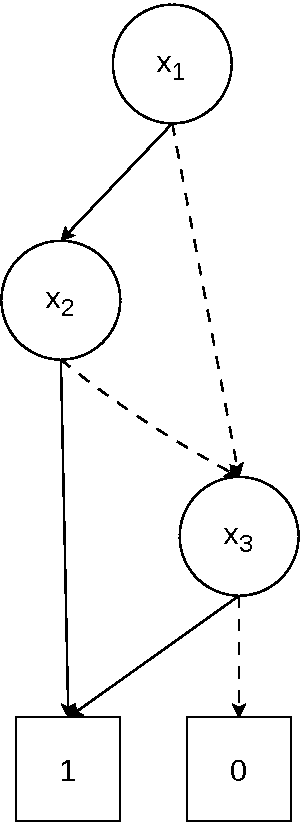
\includegraphics[width=0.22\linewidth]{figures/example-robdd.pdf}
    \caption{Reduced Ordered Binary Decision Diagram representing Boolean function $(x_1 \land x_2) \lor x_3$.}
    \label{fig:robdd}
\end{figure}

\begin{figure}
    \centering
    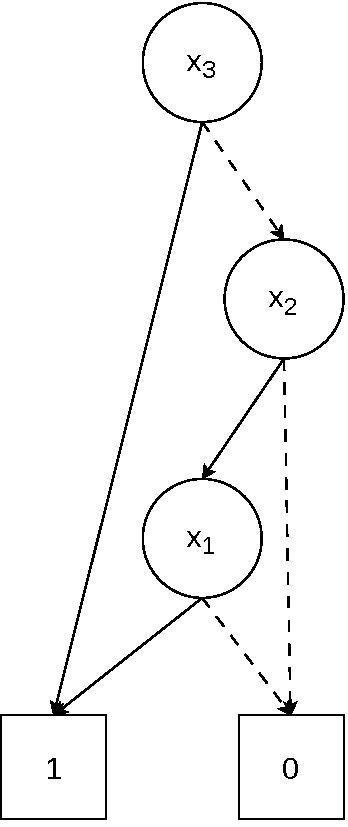
\includegraphics[width=0.25\linewidth]{figures/example-robdd-reordered.pdf}
    \caption{Reduced Ordered Binary Decision Diagram representing Boolean function $(x_1 \land x_2) \lor x_3$ with
        variable ordering reversed to the one of \ref{fig:robdd}.}
    \label{fig:robdd-reordered}
\end{figure}

There are other BDD types with further restrictions or modified properties, such as a \textit{Multi-Terminal BDD}
(MTBDD), which allows for additional leaf nodes, besides $0$ and $1$, or \textit{Multi-valued DD} (MDD) which is a
generalization of a BDD to other domains beyond the Boolean domain \cite{sylvan}. All of these types are, however,
outside the scope of this Thesis. The remainder of this text focuses exclusively on ROBDD. The terms BDD and ROBDD
will be used interchangeably from this point forward.

\section{The Apply operation}
\label{chap:bdd:apply}

A BDD is a convenient representation for satisfiability testing, equivalence checking, and performing Boolean
operations on them. Applying a Boolean operation (such as AND, OR, XOR) on two BDDs is one of the key operations of
the BDD interface \cite{bfs-bdd}. This operation, referred to as \textit{apply}, is the primary focus of this Thesis.
$apply$ takes three arguments: two BDDs and the Boolean operation. The product is then also a BDD. To better
illustrate this, consider these Boolean functions:

\begin{alignat}{1}
     f(x_1, x_2) &= x_1 \lor x_2 \label{eq:apply-a} \\
     g(x_1, x_3) &= x_1 \lor x_3 \label{eq:apply-b} \\
               h &= f \land g \label{eq:apply-result}
\end{alignat}

Function $h$ in \eqref{eq:apply-result} is the product of applying the conjunction operation to functions $f$ and
$g$. After substituting $f$ and $g$ for their definitions and simplifying the expression, we are left with  $h(x_1,
x_2, x_3) = x_1 \lor (x_2 \land x_3)$. In terms of BDD, this operation is illustrated in Figure \ref{fig:apply}.

\begin{figure}
    \centering
    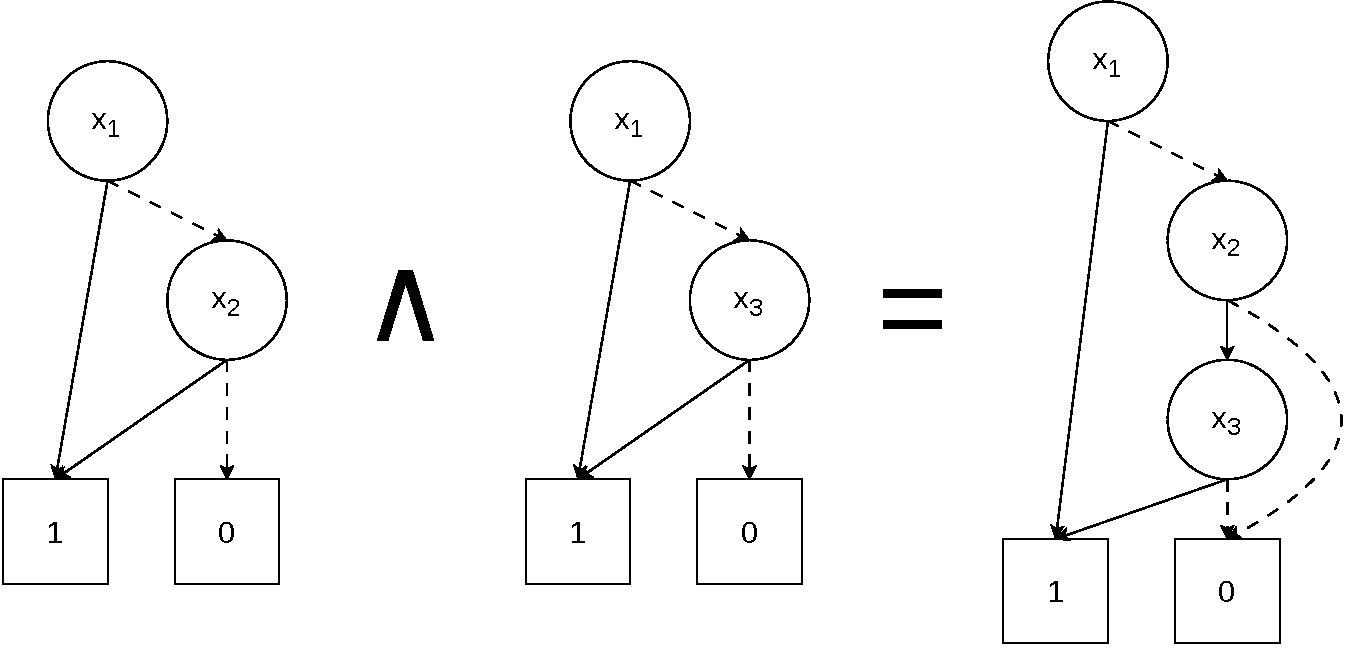
\includegraphics[width=\linewidth]{figures/example-apply.pdf}
    \caption{ROBDD produced by apply, as shown in \eqref{eq:apply-result}}
    \label{fig:apply}
\end{figure}

Most commonly, $apply$ is implemented using recursion, which is easier to demonstrate. Algorithm \ref{alg:apply}
presents the pseudocode of the $apply$ operation. $apply$ returns the root node of the resulting BDD and takes three
arguments:
\begin{enumerate}
    \item A root node of the first BDD
    \item A root node of the second BDD
    \item A Boolean operation, e.g., conjunction
\end{enumerate}

Both BDDs are traversed simultaneously in a depth-first manner from the top to the terminal nodes. Each recursive
algorithm has a base condition to stop the recursion; in this case, it is when a terminal node of each BDD is
reached. On line \ref{alg:apply:recursion-stop}, both of the nodes are used as arguments to the $op$ operation, and
the result is returned to the previous call in the call stack.

If neither or only one of the current nodes is terminal, the task cache is checked on line \ref{alg:apply:cache-get}.
This check prevents repeated computation of results that were already processed. A task cache is a commonly used
optimization that reduces the complexity class of many BDD operations from exponential time to polynomial time
\cite{sylvan}.

\begin{algorithm}
    \caption{Apply}\label{alg:apply}
    \begin{algorithmic}[1]
        \Require $node\_a$ a root node of BDD $a$
        \Require $node\_b$ a root node of BDD $b$
        \Require $op$ a Boolean operation
        \Ensure $c$ a root node of the resulting BDD
        \Function{apply}{$node\_a, node\_b, op$}
            \If{$node\_a$ is terminal AND $node\_b$ is terminal} \label{alg:apply:recursion-stop}
                \State \Return  $op(node\_a, node\_b)$
            \EndIf
            \State $chached\_res \gets cache.get(node\_a, node\_b, op)$
            \If{$cached\_res \neq null$} \label{alg:apply:cache-get}
                \State \Return $cached\_res$
            \EndIf
            \State $v \gets min(var(node\_a), var(node\_b))$ \label{alg:apply:min-var-start}
            \If{$var(node\_a) = v$}
                \State $(low\_a, high\_a) \gets (low(node\_a), high(node\_a))$
            \Else
                \State $(low\_a, high\_a) \gets (node\_a, node\_a)$
            \EndIf
            \If{$var(node\_b) = v$}
                \State $(low\_b, high\_b) \gets (low(node\_b), high(node\_b))$
            \Else
                \State $(low\_b, high\_b) \gets (node\_b, node\_b)$
            \EndIf \label{alg:apply:min-var-end}
            \State $l \gets apply(low\_a, low\_b)$ \label{alg:apply:apply-l}
            \State $h \gets apply(high\_a, high\_b)$ \label{alg:apply:apply-h}
            \If{$l \neq h$} \label{alg:apply:redundancy-check}
                \State $c \gets ensure\_node(v, l, h)$ \label{alg:apply:ensure-node}
            \Else
                \State $c \gets l$
            \EndIf
            \State $cache.put(node\_a, node\_a, op, c)$
            \State \Return $c$
        \EndFunction
    \end{algorithmic}
\end{algorithm}

For node pairs that have not been encountered before (or whose result was replaced due to the use of a lossy cache),
the algorithm selects a path to continue. Line \ref{alg:apply:min-var-start} determines which BDD to expand further;
only the BDD with a lower variable is progressed (assuming the standard variable ordering). After the low and high
node pairs of both BDDs are assigned, the $apply$ function is called recursively for both successors (lines
\ref{alg:apply:apply-l} and \ref{alg:apply:apply-h}).

Once both the low and high successors are known, the new resulting node can be created. To keep the resulting BDD
still reduced, redundant and duplicate nodes need to be eliminated. The $if$ statement on line
$\ref{alg:apply:redundancy-check}$ enforces the redundancy rule. The function $ensure\_node$ called on line
\ref{alg:apply:ensure-node} serves two purposes:
\begin{itemize}
    \item Create a new node for the given variable $v$, low successor $l$ and high successor $h$
    \item Check for duplicities and create this node if and only if it is unique to the BDD. Return an existing node
        otherwise
\end{itemize}

The final steps of the algorithm are to store the result in the task cache and return the result node. Calling
$apply$ with two root nodes and an operation yields a root node of the calculated BDD.

The recursive approach is fairly easy to understand and implement. In practice, however, recursive algorithms often
produce long stack traces and can be harder to debug, so they are not always desirable. It also reduces possibilities
for parallel execution, the main focus of this Thesis. Alternatively, recursion can be eliminated in favor of
iterative computation with supporting data structures. We will explore this more in the following subsection.

\subsection{Iterative Apply}
\label{chap:bdd:apply:iterative}

As the name implies, iterative implementation uses a loop rather than recursion. The concept of rewriting a recursive
algorithm as an iterative one is well known in Computer Science, so we will not go into exhaustive detail. The key
idea of an iterative depth-first graph traversal (DFS) is to use a last-in, first-out (LIFO) data structure --- such
as a stack.

The changes done to the $apply$ operation are minimal. During initialization, the first task is pushed into the stack
--- the node pair to be processed. The algorithm is not done if there are still tasks in the stack, so in each
iteration, an item is popped from the stack, and we loop until the stack is empty. A second stack is used to store
results.

If the task was not processed yet, push it back to the task stack with both of its successors\footnote{The same
strategy is used here as in Algorithm \ref{alg:apply} (lines \ref{alg:apply:min-var-start} through
\ref{alg:apply:min-var-end}).}. If it was processed, the first two items can be popped from the result stack because
they are the new low and high nodes.

However, implementing the same using a Breadth-first search (BFS) is significantly more difficult. The obvious
difference is using a first-in, first-out (FIFO) data structure --- such as a queue. But keeping the resulting BDD a
ROBDD requires a two-phase traversal. First, the graph is traversed from top to bottom, and all tasks are created for
later processing. This is the \textbf{expansion phase}. Here, the task cache can be replaced by ensuring that only
unique tasks are created.

The second phase (the \textbf{reduction phase}) traverses the graph from bottom up. The created tasks are processed
in reverse order of their creation. This phase is similar to the $apply$ operation we are familiar with. In this
stage, we must ensure that the node relationships are correctly aligned with the tasks that were rid of duplicities
in the previous step.

Further details are covered in Chapter \ref{chap:design}. It is clear that BFS introduces new complexity to the
operation. At the same time, it could benefit from parallel execution, in which multiple tasks are generated and
processed by multiple worker threads simultaneously. Since the algorithm now traverses the graph twice, it is
expected to perform worse than DFS implementations, but for certain inputs, this implementation might scale better.
Chapter \ref{chap:comparisons-benchmarks} covers the findings.
